\documentclass{article}
\usepackage{amsmath,amsthm}
\usepackage{amssymb,latexsym}
\usepackage{float}
\usepackage{fullpage}
\usepackage{times}

% graphs
\usepackage{tikz}
\usetikzlibrary{automata,positioning}

\tikzset{initial text={}}

\newtheorem{theorem}{Theorem}
\newtheorem{corollary}[theorem]{Corollary}
\newtheorem{question}[theorem]{Question}
\newtheorem{lemma}[theorem]{Lemma}
\newtheorem{observation}[theorem]{Observation}
\newtheorem{proposition}{Proposition}
\newtheorem{definition}[theorem]{Definition}
\newtheorem{claim}[theorem]{Claim}
\newtheorem{fact}[theorem]{Fact}
\newtheorem{assumption}[theorem]{Assumption}
\newtheorem{example}{Example}
\newtheorem{conjecture}[theorem]{Conjecture}
\newtheorem{alg}[theorem]{Algorithm}

\newcommand{\set}[1]{{\left\{#1\right\}}}    % braces for set notation
\newcommand{\ve}[1]{\mathbf{#1}}
\newcommand{\abs}[1]{\left\lvert #1 \right\rvert}
\newcommand{\poly}{\operatorname{poly}}
\newcommand{\complex}{{\mathbb C}}
\newcommand{\reals}{{\mathbb R}}
\newcommand{\ints}{{\mathbb Z}}
\newcommand{\nats}{{\mathbb N}}
\newcommand{\proj}[1]{\mbox{$|#1\rangle \!\langle #1 |$}}
\newcommand{\enc}[1]{\left<#1\right>}
\newcommand{\spa}[1]{\mathcal{#1}}
\newcommand{\ayes}{A_{\rm yes}}
\newcommand{\ano}{A_{\rm no}}

\begin{document}

\title{
    CMSC 303 Introduction to Theory of Computation, VCU\\
    Assignment: 3\\
    Name: Steven Hernandez
}

\date{}

\maketitle
\vspace{-10mm}

\begin{enumerate}
    \item % 1
        \begin{enumerate}
            \item
                $R_a = 0\Sigma^*1$

                Which says: $0$ concatenated with zero or more character concatenated with 1.
            \item
                $R_b = (\Sigma^*0\Sigma^*)^4$

                Says: zero or more characters followed by a $0$ follower by zero or more of any character, which is then repeated 4 times.
            \item
                $R_c = 1 \bigcup 11 \bigcup \epsilon$

                Which explicitly states the contents of the language.
            \item
                $R_d = \set{\Sigma} \bigcup \set{\Sigma\Sigma} \bigcup \set{\Sigma\Sigma\Sigma} \bigcup \set{\epsilon}$

                Explicitly allows for any strings with one character or two characters or three characters of no characters.
            \item
                $R_e = $ % TODO
            \item
                $R_f = \Sigma^+$

                Plus indicates 1 or more.
        \end{enumerate}
    \item % 2
        \begin{enumerate}
            \item
                $M_a = (Q, \Sigma, \delta, q, F)$ such that:

                \[  Q = \set{q_0} \\
                    \Sigma is our language \\
                    q = q_0 \\
                    F = \set{q_0} \\
                    \delta = \epsilon
                \]
                because any transitions would mean a character was read, which would not be a part of the language we are looking for.
            \item
                $M_b = (Q, \Sigma, \delta, q, F)$ such that:

                \[  Q = \set{q_0, q_1, q_2, q_3} \\
                    q = q_0 \\
                    F = \set{q_3} \\
                \]

                Define $\delta$ by:

                \begin{tabular}{|c | c   c|}
                    \hline
                    $\delta$ & 0      & 1 \\
                    \hline
                    $q_0$    & $q_0$  & $q_1$ \\
                    $q_1$    & $q_0$  & $q_2$ \\
                    $q_2$    & $q_0$  & $q_3$ \\
                    $q_3$    & $q_3$  & $q_3$ \\
                    \hline
                \end{tabular}
        \end{enumerate}
    \item % 3
        State Diagram for $M$:

        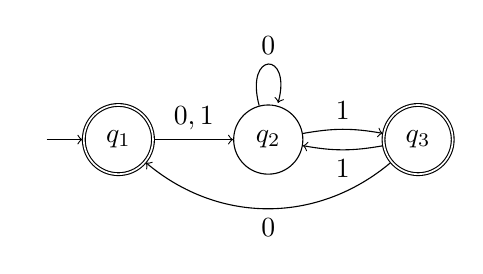
\begin{tikzpicture}
           \node[state,initial,accepting] (q_1)   {$q_1$};
           \node[state] (q_2) [right=of q_1] {$q_2$};
           \node[state,accepting] (q_3) [right=of q_2] {$q_3$};
            \path[->]
            (q_1) edge [above] node {$0,1$} (q_2)
            (q_2) edge [loop above] node {$0$} (q_2)
                  edge [bend left=10, above] node {$1$} (q_3)
            (q_3) edge [bend left=40, below] node {$0$} (q_1)
                  edge [bend left=10, below] node {$1$} (q_2);
        \end{tikzpicture}

        Steps for reaching regular expression for $M$:

        \begin{enumerate}
            \item
                Add $q_{start}$ and $q_{end}$ as explained in Lemma 1.60

                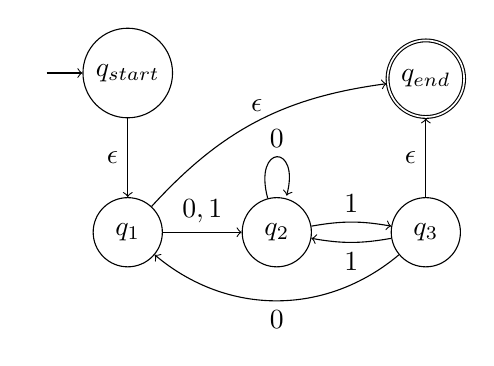
\begin{tikzpicture}
                   \node[state,initial] (q_start)   {$q_{start}$};
                   \node[state] (q_1) [below=of q_start] {$q_1$};
                   \node[state] (q_2) [right=of q_1] {$q_2$};
                   \node[state] (q_3) [right=of q_2] {$q_3$};
                   \node[state,accepting] (q_end) [above=of q_3] {$q_{end}$};
                    \path[->]
                    (q_start) edge [left] node {$\epsilon$} (q_1)
                    (q_1) edge [above] node {$0,1$} (q_2)
                          edge [bend left=20, above] node {$\epsilon$} (q_end)
                    (q_2) edge [loop above] node {$0$} (q_2)
                          edge [bend left=10, above] node {$1$} (q_3)
                    (q_3) edge [bend left=40, below] node {$0$} (q_1)
                          edge [bend left=10, below] node {$1$} (q_2)
                          edge [left] node {$\epsilon$} (q_end);
                \end{tikzpicture}
            \item
                Update each transition to a regular expression.

                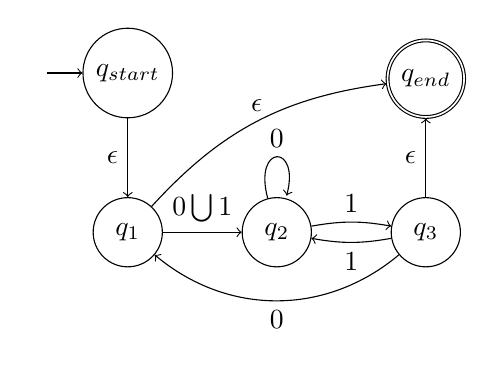
\begin{tikzpicture}
                   \node[state,initial] (q_start)   {$q_{start}$};
                   \node[state] (q_1) [below=of q_start] {$q_1$};
                   \node[state] (q_2) [right=of q_1] {$q_2$};
                   \node[state] (q_3) [right=of q_2] {$q_3$};
                   \node[state,accepting] (q_end) [above=of q_3] {$q_{end}$};
                    \path[->]
                    (q_start) edge [left] node {$\epsilon$} (q_1)
                    (q_1) edge [above] node {$0\bigcup1$} (q_2)
                          edge [bend left=20, above] node {$\epsilon$} (q_end)
                    (q_2) edge [loop above] node {$0$} (q_2)
                          edge [bend left=10, above] node {$1$} (q_3)
                    (q_3) edge [bend left=40, below] node {$0$} (q_1)
                          edge [bend left=10, below] node {$1$} (q_2)
                          edge [left] node {$\epsilon$} (q_end);
                \end{tikzpicture}
            \item
                $q_{rip}=q_2$

                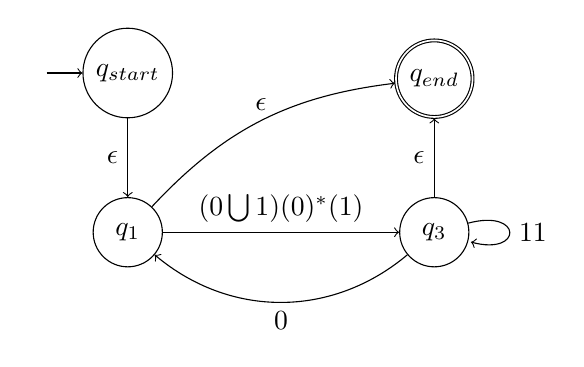
\begin{tikzpicture}
                   \node[state,initial] (q_start)   {$q_{start}$};
                   \node[state] (q_1) [below=of q_start] {$q_1$};
                   \node[state] (q_3) [right=3cm of q_1] {$q_3$};
                   \node[state,accepting] (q_end) [above=of q_3] {$q_{end}$};
                    \path[->]
                    (q_start) edge [left] node {$\epsilon$} (q_1)
                    (q_1) edge [above] node {$(0\bigcup1)(0)^*(1)$} (q_3)
                          edge [bend left=20, above] node {$\epsilon$} (q_end)
                    (q_3) edge [bend left=40, below] node {$0$} (q_1)
                          edge [loop right] node {$11$} (q_3)
                          edge [left] node {$\epsilon$} (q_end);
                \end{tikzpicture}
            \item
                Simplified to:

                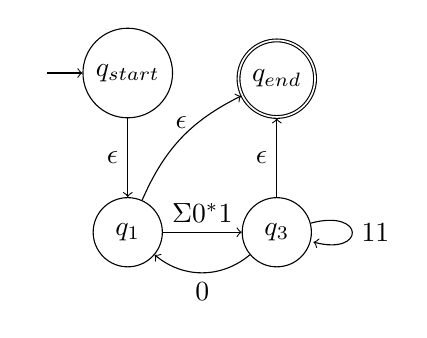
\begin{tikzpicture}
                   \node[state,initial] (q_start)   {$q_{start}$};
                   \node[state] (q_1) [below=of q_start] {$q_1$};
                   \node[state] (q_3) [right=of q_1] {$q_3$};
                   \node[state,accepting] (q_end) [above=of q_3] {$q_{end}$};
                    \path[->]
                    (q_start) edge [left] node {$\epsilon$} (q_1)
                    (q_1) edge [above] node {$\Sigma0^*1$} (q_3)
                          edge [bend left=20, above] node {$\epsilon$} (q_end)
                    (q_3) edge [bend left=40, below] node {$0$} (q_1)
                          edge [loop right] node {$11$} (q_3)
                          edge [left] node {$\epsilon$} (q_end);
                \end{tikzpicture}
            \item
                $q_{rip}=q_3$

                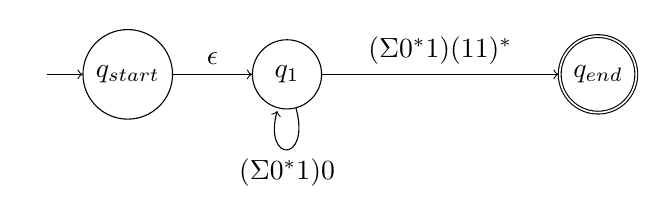
\begin{tikzpicture}
                   \node[state,initial] (q_start)   {$q_{start}$};
                   \node[state] (q_1) [right=of q_start] {$q_1$};
                   \node[state,accepting] (q_end) [right=3cm of q_1] {$q_{end}$};
                    \path[->]
                    (q_start) edge [above] node {$\epsilon$} (q_1)
                    (q_1) edge [loop below] node {$(\Sigma0^*1)0$} (q_1)
                          edge [above] node {$(\Sigma0^*1)(11)^*$} (q_end);
                \end{tikzpicture}
            \item
                $q_{rip}=q_1$

                \begin{tikzpicture}
                   \node[state,initial] (q_start)   {$q_{start}$};
                   \node[state,accepting] (q_end) [right=3cm of q_1] {$q_{end}$};
                    \path[->]
                    (q_start) edge [above] node {$((\Sigma0^*1)0)^*(\Sigma0^*1)(11)^*$} (q_end);
                \end{tikzpicture}

                Thus our regular expression is $((\Sigma0^*1)0)^*(\Sigma0^*1)(11)^*$.
        \end{enumerate}
    \item % 4
        \begin{enumerate}
            \item
            \item
            \item
        \end{enumerate}
    \item % 5
        \begin{enumerate}
            \item
            \item
        \end{enumerate}
\end{enumerate}

\end{document}
